\documentclass{subfiles}
\begin{document}
\begin{figure}[!h]
    \centering
    \begin{subfigure}[b]{0.4\textwidth}
        \centering
        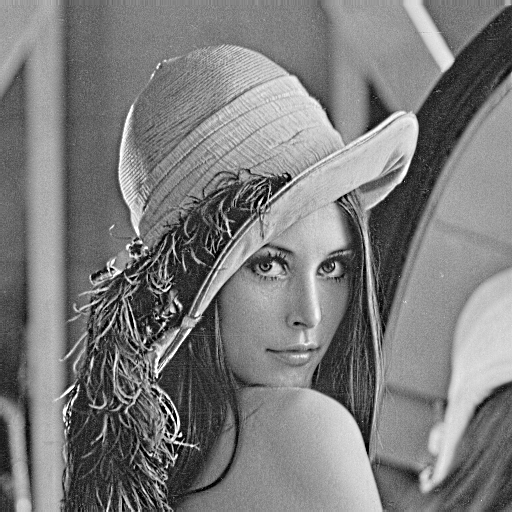
\includegraphics[scale = 0.3]{../Images/Lena/Lena con operatore kappa.png}
        \caption{Operatore kappa applicato a LenaGS.}
    \end{subfigure}
    \hspace{10pt}
    \begin{subfigure}[b]{0.4\textwidth}
        \centering
        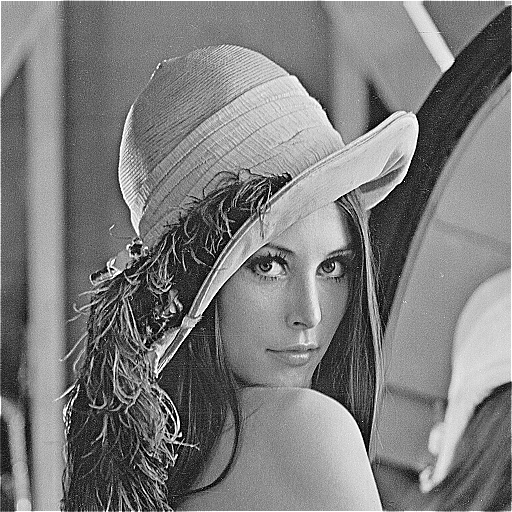
\includegraphics[scale = 0.3]{../Images/Lena/SharpnedLena.png}
        \caption{Filtro gradiente applicato a LenaGS.}
    \end{subfigure}
    \caption{Esemplificazione della similarità tra l'operatore morfologico kappa e filtro di sharpening.}
    \label{fig:7.4}
\end{figure}
\end{document}